\documentclass{beamer}
\usetheme{metropolis}
\usepackage{../../resources/style}

\newcommand{\beginnote}[1]{%
  \vfill
  {\footnotesize\textcolor{gray}{\textit{$\triangleright$ #1 (vezi slide-ul \emph{Resurse})}}}%
}

\title{Căutare binară}
% pentru clasa a 6-a (sectiunile 5-6 comentate):
% \subtitle{Varianta clasică $\cdot$ Variații $\cdot$ STL $\cdot$ Complexitate}
% pentru clasa a 9-a:
\subtitle{Varianta clasică $\cdot$ Variații $\cdot$ STL $\cdot$ Complexitate \\ Căutare binară pe rezultat}
\author{Andrei Mihai Ciobanu}
\institute{Algolymp Summer School}
\date{}
\titlegraphic{
\includegraphics[width=4cm]{../../resources/algolymp-logo.png}}
\setbeamertemplate{frame footer}{Algolymp Summer School}

% ----------------------------------------------------------------
\begin{document}

\begin{frame}[shrink]
  \titlepage
\end{frame}

\begin{frame}{Cuprins}
  \tableofcontents
\end{frame}

% ================================================================
% SECTIUNEA 1
% ================================================================
\section{Căutarea binară a unui element}

\begin{frame}{Motivație}
  \textbf{Problemă:} avem un șir \emph{sortat} cu $n$ elemente și vrem să știm dacă valoarea $x$ se află în el.

  \textbf{Căutare secvențială:} parcurgem elementele pe rând $\rightarrow$ în cel mai rău caz, $n$ comparații.

  \textbf{Căutare binară:} folosim faptul că șirul e sortat și eliminăm jumătate din elemente la fiecare pas.

  \smallskip
  \begin{center}
  \begin{tabular}{lcc}
    \toprule
    $n$ & Secvențial & Binar \\
    \midrule
    $10$            & $10$ pași       & $4$ pași  \\
    $100$           & $100$ pași      & $7$ pași  \\
    $1\,000\,000$   & $10^6$ pași     & $20$ pași \\
    \bottomrule
  \end{tabular}
  \end{center}
\end{frame}

\begin{frame}{Idee}
  \begin{block}{Condiții}
    \begin{itemize}
      \item Șirul trebuie să fie \textbf{sortat} (crescător sau descrescător)
      %\item Acces direct la element prin indice în $O(1)$ (tablou / \texttt{vector})
    \end{itemize}
  \end{block}

  \smallskip
  Păstrăm un interval $[st, dr]$ care conține răspunsul. La fiecare pas:
  \begin{enumerate}
    \item Calculăm mijlocul: $mij = (st + dr) \ / \ 2$
    \item Comparăm $v[mij]$ cu $x$:
    \begin{itemize}
      \item $v[mij] = x$ $\rightarrow$ \textbf{găsit!}
      \item $v[mij] < x$ $\rightarrow$ $st = mij + 1$ \textemdash{} căutăm în dreapta
      \item $v[mij] > x$ $\rightarrow$ $dr = mij - 1$ \textemdash{} căutăm în stânga
    \end{itemize}
  \end{enumerate}
  \smallskip
  Ne oprim când găsim valoarea sau când intervalul devine gol ($st > dr$).
\end{frame}

\begin{frame}{Algoritm pas cu pas}
  Șir sortat: $v = [2,\ 5,\ 8,\ 11,\ 14,\ 17,\ 20,\ 23,\ 26,\ 29,\ 32]$, căutăm $x = 23$.

  \smallskip
  \begin{itemize}
    \item $st=0,\;dr=10 \Rightarrow mij=5,\;v[5]=17 < 23 \Rightarrow st = 6$
    \item $st=6,\;dr=10 \Rightarrow mij=8,\;v[8]=26 > 23 \Rightarrow dr = 7$
    \item $st=6,\;dr=7\;\;\Rightarrow mij=6,\;v[6]=20 < 23 \Rightarrow st = 7$
    \item $st=7,\;dr=7\;\;\Rightarrow mij=7,\;v[7]=23 = 23 \Rightarrow$ \textbf{găsit la poziția $7$} \checkmark
  \end{itemize}
\end{frame}

\begin{frame}{Vizualizare \textemdash{} intervalul se înjumătățește}
  \begin{center}
  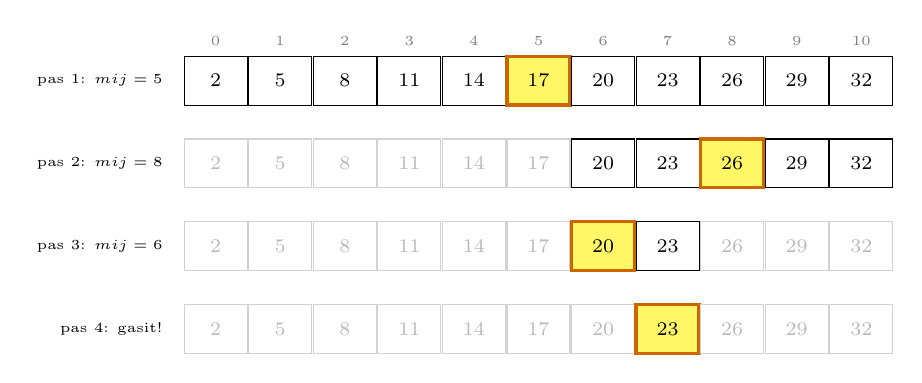
\begin{tikzpicture}[
      box/.style={draw, minimum width=0.8cm, minimum height=0.62cm, font=\scriptsize},
      lbl/.style={font=\tiny}
    ]
    \foreach \i/\val in {0/2,1/5,2/8,3/11,4/14,5/17,6/20,7/23,8/26,9/29,10/32} {
      \node[lbl, text=gray] at (\i*0.82, 0.5) {\i};
    }
    \foreach \r/\st/\dr/\mij/\txt in {0/0/10/5/{pas 1: $mij=5$},1/6/10/8/{pas 2: $mij=8$},2/6/7/6/{pas 3: $mij=6$},3/7/7/7/{pas 4: gasit!}} {
      \node[lbl, anchor=east] at (-0.55, -1.05*\r) {\txt};
      \foreach \i/\val in {0/2,1/5,2/8,3/11,4/14,5/17,6/20,7/23,8/26,9/29,10/32} {
        \ifnum\i<\st
          \node[box, draw=gray!35, text=gray!55] at (\i*0.82, -1.05*\r) {\val};
        \else
          \ifnum\i>\dr
            \node[box, draw=gray!35, text=gray!55] at (\i*0.82, -1.05*\r) {\val};
          \else
            \ifnum\i=\mij
              \node[box, fill=yellow!60, very thick, draw=orange!80!black] at (\i*0.82, -1.05*\r) {\val};
            \else
              \node[box] at (\i*0.82, -1.05*\r) {\val};
            \fi
          \fi
        \fi
      }
    }
  \end{tikzpicture}
  \end{center}
  \smallskip
  La fiecare pas, intervalul $[st, dr]$ se \textbf{înjumătățește}.
\end{frame}

\begin{frame}[fragile, shrink]{Căutare secvențială \textemdash{} implementare}
  \begin{lstlisting}
int n, x;
cin >> n >> x;
vector<int> v(n);
for (int i = 0; i < n; i++) {
    cin >> v[i];
}

int poz = -1;
for (int i = 0; i < n; i++) {
    if (v[i] == x) {
        poz = i;
        break;
    }
}

cout << poz;
  \end{lstlisting}
  \begin{itemize}
    \item Complexitate: $O(n)$ \textemdash{} în cel mai rău caz parcurgem tot șirul
    \item Funcționează pe orice șir, \textbf{sortat sau nu}
  \end{itemize}
\end{frame}

\begin{frame}[fragile, shrink]{Căutare binară \textemdash{} implementare}
  \begin{lstlisting}
int n, x;
cin >> n >> x;
vector<int> v(n);
for (int i = 0; i < n; i++) {
    cin >> v[i];
}

int st = 0, dr = n - 1, poz = -1;
while (st <= dr) {
    int mij = (st + dr) / 2;
    if (v[mij] == x) {
        poz = mij;
        break;
    } else if (v[mij] < x) {
        st = mij + 1;  // cautam in dreapta
    } else {
        dr = mij - 1;  // cautam in stanga
    }
}

cout << poz;
  \end{lstlisting}
  \begin{itemize}
    \item Complexitate: $O(\log n)$ \textemdash{} \textbf{șirul trebuie să fie sortat}
  \end{itemize}
\end{frame}

% ================================================================
% SECTIUNEA 2
% ================================================================
\section{Variații}

\begin{frame}{Lower bound \textemdash{} upper bound}
  Căutarea clasică găsește \textbf{o apariție oarecare} a lui $x$. Adesea avem nevoie de:

  \smallskip
  \begin{itemize}
    \item \textbf{Lower bound:} prima poziție cu $v[poz] \geq x$
    \item \textbf{Upper bound:} prima poziție cu $v[poz] > x$
  \end{itemize}

  Exemplu: $v = [1,\ 2,\ 2,\ 2,\ 3,\ 5]$, $x = 2$

  \smallskip
  \begin{center}
  \begin{tabular}{lcc}
    \toprule
    & Poziție & Valoare \\
    \midrule
    Lower bound ($\geq 2$) & $1$ & $v[1] = 2$ \\
    Upper bound ($> 2$)    & $4$ & $v[4] = 3$ \\
    \bottomrule
  \end{tabular}
  \end{center}

  \smallskip
  Numărul de apariții ale lui $x$: $\text{upper\_bound} - \text{lower\_bound} = 4 - 1 = 3$
\end{frame}

\begin{frame}[fragile]{Implementare \texttt{lower\_bound}}
  \begin{lstlisting}
// prima pozitie cu v[poz] >= x
// rez = n daca toate elementele < x
int st = 0, dr = n - 1, rez = n;
while (st <= dr) {
    int mij = (st + dr) / 2;
    if (v[mij] >= x) {
        rez = mij;    // candidat, continuam in stanga
        dr = mij - 1;
    } else {
        st = mij + 1;
    }
}
  \end{lstlisting}
  Când $v[mij] \geq x$, \textbf{salvăm} poziția și căutăm mai la stânga un candidat mai bun.
\end{frame}

\begin{frame}[fragile]{Implementare \texttt{upper\_bound}}
  \begin{lstlisting}
// prima pozitie cu v[poz] > x
// rez = n daca toate elementele <= x
int st = 0, dr = n - 1, rez = n;
while (st <= dr) {
    int mij = (st + dr) / 2;
    if (v[mij] > x) {
        rez = mij;    // candidat, continuam in stanga
        dr = mij - 1;
    } else {
        st = mij + 1;
    }
}
  \end{lstlisting}
  Singura diferență față de \texttt{lower\_bound}: condiția \lstinline|v[mij] > x| în loc de \lstinline|v[mij] >= x|.
\end{frame}

\begin{frame}[fragile, shrink]{Ultima poziție cu $v[poz] < x$ / $\leq x$}
  Aceleași idei ne dau și pozițiile din partea cealaltă:
  \begin{itemize}
    \item Ultima poziție cu $v[poz] < x$ $=$ \texttt{lower\_bound}$(x) - 1$
    \item Ultima poziție cu $v[poz] \leq x$ $=$ \texttt{upper\_bound}$(x) - 1$
  \end{itemize}
  Sau adaptăm direct implementarea, inversând sensul căutării:
  \begin{lstlisting}
// ultima pozitie cu v[poz] <= x
// rez = -1 daca toate elementele > x
int st = 0, dr = n - 1, rez = -1;
while (st <= dr) {
    int mij = (st + dr) / 2;
    if (v[mij] <= x) {
        rez = mij;    // candidat, continuam in dreapta
        st = mij + 1;
    } else {
        dr = mij - 1;
    }
}
  \end{lstlisting}
  Pentru $< x$: schimbăm condiția în \lstinline|v[mij] < x|.
\end{frame}

% ================================================================
% SECTIUNEA 3
% ================================================================
\section{Variații în STL}

\begin{frame}[fragile, shrink]{STL: \texttt{binary\_search}, \texttt{lower\_bound}, \texttt{upper\_bound}}
  C++ oferă aceste funcții gata implementate în \lstinline|<algorithm>|, toate $O(\log n)$:
  \begin{lstlisting}
#include <algorithm>
vector<int> v = {1, 2, 2, 2, 3, 5};

// Exista x in v? (true/false)
bool exista = binary_search(v.begin(), v.end(), 2);

// Iteratori
auto it1 = lower_bound(v.begin(), v.end(), 2);
auto it2 = upper_bound(v.begin(), v.end(), 2);

// Pozitii (indici)
int poz1 = it1 - v.begin(); // poz1 = 1 (prima aparitie)
int poz2 = it2 - v.begin(); // poz2 = 4 (dupa ultima)

// Numarul de aparitii ale lui x
int cate = it2 - it1;       // cate = 3
  \end{lstlisting}
  \beginnote{vector, iterator \textemdash{} din STL}
\end{frame}

\begin{frame}[fragile]{STL \textemdash{} numărare pe interval $[x, y]$}
  \begin{lstlisting}
vector<int> v = {23, 2, 5, 26, 11, 17, 14, 8, 20};
// sirul trebuie sortat inainte!
sort(v.begin(), v.end());

int x = 8, y = 20;

// prima pozitie cu v[poz] >= x
int st = lower_bound(v.begin(), v.end(), x) - v.begin();

// prima pozitie cu v[poz] > y
int dr = upper_bound(v.begin(), v.end(), y) - v.begin();

int cate = dr - st; // cate = 5  (8, 11, 14, 17, 20)
  \end{lstlisting}
  \begin{itemize}
    \item Idee frecventă: interogări pe șir sortat în $O(\log n)$ în loc de $O(n)$
  \end{itemize}
\end{frame}

% ================================================================
% SECTIUNEA 4
% ================================================================
\section{De ce $O(\log n)$?}

\begin{frame}{De ce $O(\log n)$?}
  La fiecare pas, intervalul $[st, dr]$ se \textbf{înjumătățește}:
  \[
    n \;\to\; \frac{n}{2} \;\to\; \frac{n}{4} \;\to\; \cdots \;\to\; 1
  \]
  Numărul de pași până ajungem la $1$: $\log_2 n$.

  \smallskip
  \begin{center}
  \begin{tabular}{lcc}
    \toprule
    $n$ & $\log_2 n$ & Pași maximi \\
    \midrule
    $10$              & $3.32$   & $4$  \\
    $1\,000$          & $9.97$   & $10$ \\
    $10^6$            & $19.93$  & $20$ \\
    $10^9$            & $29.90$  & $30$ \\
    $10^{18}$         & $59.79$  & $60$ \\
    \bottomrule
  \end{tabular}
  \end{center}

  \smallskip
  Chiar și pentru $n = 10^{18}$, avem cel mult $60$ de pași!
\end{frame}

% ================================================================
% SECTIUNILE 5-6: decomentati pentru clasa a 9-a
% (decomentati si randul din tabelul de Recapitulare)
% ================================================================

\section{Căutare binară pe rezultat}

\begin{frame}{Căutare binară pe rezultat \textemdash{} exemplu}
  Cea mai puternică aplicație: nu căutăm o valoare într-un șir, ci \textbf{cel mai bun răspuns posibil}.

  \smallskip
  \begin{block}{Problemă}
    Avem $n$ bețe de lungimi $d_1, d_2, \dots, d_n$. Fiecare băț poate fi tăiat în bucăți mai mici de lungimi întregi. Determinați \textbf{lungimea maximă} $L$ pentru care obținem în total \textbf{cel puțin} $A$ bucăți.
  \end{block}

  \smallskip
  Restricții: $1 \leq n \leq 10^5$, $1 \leq d_i \leq 10^9$, $1 \leq A \leq 10^9$.

  Exemplu: $d = [7,\ 4,\ 9,\ 5]$, $A = 6$ $\Rightarrow$ răspuns $L = 3$ (obținem $2+1+3+1 = 7 \geq 6$ bucăți).
\end{frame}

\begin{frame}[fragile, shrink]{Căutare binară pe rezultat \textemdash{} soluție naivă}
  Cea mai simplă idee: încercăm pe rând fiecare lungime posibilă, de la cea mai mare la cea mai mică, și ne oprim la prima care funcționează.
  \begin{lstlisting}
long long taieBucati(vector<int>& d, int L) {
    long long bucati = 0;
    for (int i = 0; i < d.size(); ++i) {
        bucati += d[i] / L;
    }
    return bucati;
}

for (int L = maxim; L >= 1; L--) {
    if (taieBucati(d, L) >= A) {
        cout << L;
        break;
    }
}
  \end{lstlisting}
  \begin{itemize}
    \item Complexitate: $O(n \cdot maxim)$, unde $maxim$ este lungimea maximă a unui băț
    \item Pentru $maxim = 10^9$ și $n = 10^5$: mult prea lent
  \end{itemize}
\end{frame}

\begin{frame}{Căutare binară pe rezultat \textemdash{} observație}
  Pe măsură ce $L$ crește, numărul de bucăți obținute de \lstinline|taieBucati(d, L)| \textbf{scade} (sau rămâne la fel).

  Exemplu: $d = [7,\ 4,\ 9,\ 5]$, verificăm $taieBucati(L) \geq A$, $A = 6$

  \smallskip
  \begin{center}
  \begin{tabular}{lccccccccc}
    \toprule
    $L$                & 1  & 2  & 3 & 4 & 5 & 6 & 7 & 8 & 9 \\
    \midrule
    $taieBucati(L)$    & 25 & 11 & 7 & 5 & 3 & 2 & 2 & 1 & 1 \\
    $\geq A$?          & \checkmark & \checkmark & \checkmark & $\times$ & $\times$ & $\times$ & $\times$ & $\times$ & $\times$ \\
    \bottomrule
  \end{tabular}
  \end{center}

  \smallskip
  \begin{block}{Observație}
    Șirul de valori $taieBucati(L)$ e \textbf{monoton descrescător}: odată ce scade sub $A$, rămâne sub $A$. Îl putem privi ca pe un șir sortat descrescător (la fel ca la $lower\_bound$, vezi secțiunea \emph{Variații}) și \textbf{eliminăm jumătate din candidați} la fiecare iterație.
  \end{block}
\end{frame}

\begin{frame}[fragile, shrink]{Căutare binară pe rezultat \textemdash{} soluție optimizată}
  \begin{lstlisting}
long long taieBucati(vector<int>& d, int L) {
    long long bucati = 0;
    for (int i = 0; i < d.size(); ++i) {
        bucati += d[i] / L;
    }
    return bucati;
}

int st = 1, dr = maxim, rez = 0;
while (st <= dr) {
    int mij = (st + dr) / 2;
    if (taieBucati(d, mij) >= A) {
        rez = mij;     // functioneaza, incercam mai mare
        st = mij + 1;
    } else {
        dr = mij - 1;  // nu functioneaza, incercam mai mic
    }
}
cout << rez;
  \end{lstlisting}
  \begin{itemize}
    \item Complexitate: $O(n \log(maxim))$ \textemdash{} pentru aceleași date, $\approx 10^5 \cdot 30 = 3 \times 10^6$
  \end{itemize}
\end{frame}

\begin{frame}{Căutare binară pe rezultat \textemdash{} observație: overflow}
  \begin{block}{Observație: overflow}
    La căutarea binară pe rezultat, intervalul $[st, dr]$ poate fi foarte mare (de exemplu $dr = maxim \approx 10^9$), deci $st + dr$ riscă să depășească un \lstinline|int|.

    În astfel de cazuri, ori folosim \lstinline|long long| pentru $st$, $dr$, $mij$, ori schimbăm formula pentru mijloc: \lstinline[keepspaces=true]|mij = st + (dr - st) / 2|.
  \end{block}

  \smallskip
  Comparativ, la căutarea binară a unui element, $[st, dr]$ e mărginit de $n$ (indici de tablou), deci acest risc de overflow nu apare de obicei.
\end{frame}

\begin{frame}{Căutare binară pe rezultat \textemdash{} condiția de aplicabilitate}
  Căutarea binară pe rezultat funcționează \textbf{doar} când există o structură de tipul:

  \smallskip
  \begin{center}
  \begin{tabular}{ccccccccc}
    $\ldots$ & \checkmark & \checkmark & \checkmark & \textbf{$\times$} & $\times$ & $\times$ & $\times$ & $\ldots$ \\
  \end{tabular}
  \end{center}

  \smallskip
  adică există un \textbf{singur prag} unde condiția $taieBucati(L) \geq A$ trece din adevărat în fals (sau invers) \textemdash{} exact ca în tabelul de la exemplul cu bețele.
\end{frame}

\begin{frame}{Căutare binară pe rezultat \textemdash{} verificare practică}
  \begin{block}{Verificare practică}
    Înainte să aplici căutarea binară pe rezultat: întreabă-te \emph{``pentru \textbf{orice} $L$ care merge, merge și $L-1$?''}
    Dacă da pentru toate valorile, funcția e monotonă și poți aplica căutarea binară.
  \end{block}

  \smallskip
  \begin{block}{Exemple care \textbf{nu} respectă condiția}
    \begin{itemize}
      \item Șir nesortat $\Rightarrow$ nu poți aplica căutarea binară pe element
      \item Funcție de tip \checkmark $\times$ \checkmark $\times$ \checkmark $\Rightarrow$ nu e monotonă
    \end{itemize}
  \end{block}
\end{frame}

% ================================================================
\section{Recapitulare}

\begin{frame}{Recapitulare}
  \begin{center}
  \begin{tabular}{lll}
    \toprule
    Variantă & Timp & Spațiu \\
    \midrule
    Căutare secvențială              & $O(n)$      & $O(1)$ \\
    Căutare binară (element)         & $O(\log n)$ & $O(1)$ \\
    STL \texttt{lower/upper\_bound}  & $O(\log n)$ & $O(1)$ \\
    Căutare binară pe rezultat     & $O(\log n \cdot f(n))$ & depinde \\ 
    \bottomrule
  \end{tabular}
  \end{center}

  \smallskip
  \begin{itemize}
    \item Șirul trebuie sortat înainte de căutare binară
    \item Pentru intervale $[st, dr]$ foarte mari, folosim \lstinline|long long| sau formula sigură \lstinline[keepspaces=true]|mij = st + (dr - st) / 2|
    \item \texttt{lower\_bound} $\rightarrow$ prima poz. cu $\geq x$; \texttt{upper\_bound} $\rightarrow$ prima poz. cu $> x$
  \end{itemize}
\end{frame}

% ================================================================
\section{Resurse}

\begin{frame}{Resurse}
  \begin{block}{Română}
    \begin{itemize}\footnotesize\itemsep0pt
      \item \href{https://www.pbinfo.ro/articole/3633/cautarea-binara}{\textbf{pbinfo.ro}} \textemdash{} Căutarea binară (RO)
      \item \href{https://infoas.ro/lectie/122/cautare-binara-in-c}{\textbf{infoas.ro}} \textemdash{} Căutare binară în C++ (RO)
    \end{itemize}
  \end{block}
  \vspace{-6pt}
  \begin{block}{Engleză}
    \begin{itemize}\footnotesize\itemsep0pt
      \item \href{https://cp-algorithms.com/num_methods/binary_search.html}{\textbf{cp-algorithms.com}} \textemdash{} Binary Search (EN, detaliat, include și căutarea binară pe numere reale)
      \item \href{https://usaco.guide/silver/binary-search}{\textbf{usaco.guide}} \textemdash{} Binary Search on Monotonic Functions (EN)
      % \item \href{https://www.geeksforgeeks.org/dsa/binary-search/}{\textbf{geeksforgeeks.org}} \textemdash{} Binary Search (EN)
      % \item \href{https://www.w3schools.com/dsa/dsa_algo_binarysearch.php}{\textbf{w3schools.com}} \textemdash{} Binary Search cu simulare (EN)
      % \item \href{https://en.wikipedia.org/wiki/Binary_search}{\textbf{wikipedia.org}} \textemdash{} Binary search, istoric (EN)
    \end{itemize}
  \end{block}
  \vspace{-6pt}
  \begin{block}{Documentație C++}
    \begin{itemize}\footnotesize\itemsep0pt
      \item \href{https://en.cppreference.com/w/cpp/algorithm/lower_bound.html}{\textbf{cppreference.com}} \textemdash{} \texttt{lower\_bound} / \texttt{upper\_bound}
    \end{itemize}
  \end{block}
  \vspace{-6pt}
  \begin{block}{Fun fact}
    \begin{itemize}\footnotesize\itemsep0pt
      \item \href{https://cp-algorithms.com/num_methods/ternary_search.html}{\textbf{cp-algorithms.com}} \textemdash{} Ternary Search (EN) \textemdash{} căutare \textbf{ternară}, folosită pentru funcții unimodale (ex. $ax^2+bx+c$)
    \end{itemize}
  \end{block}
\end{frame}

% ================================================================
\section{Probleme de antrenament}

\begin{frame}{Probleme de antrenament}
  \begin{block}{Ușoare}
    \begin{itemize}\footnotesize\itemsep0pt
      \item \href{https://code.algolymp.com/problems/3963}{\textbf{Classic Binary Search \#3963}} {\footnotesize\textcolor{gray}{(AlgoCode)}}
      \item \href{https://code.algolymp.com/problems/4202}{\textbf{First Position Not Less Than Query \#4202}} {\footnotesize\textcolor{gray}{(AlgoCode)}}
    \end{itemize}
  \end{block}
  \vspace{-4pt}
  \begin{block}{Medii}
    \begin{itemize}\footnotesize\itemsep0pt
      \item \href{https://code.algolymp.com/problems/1009}{\textbf{Search Task \#1009}} {\footnotesize\textcolor{gray}{(AlgoCode)}}
      \item \href{https://code.algolymp.com/problems/3962}{\textbf{Snack Route \#3962}} {\footnotesize\textcolor{gray}{(AlgoCode)}}
    \end{itemize}
  \end{block}
  \vspace{-4pt}
  \begin{block}{Grea}
    \begin{itemize}\footnotesize\itemsep0pt
      \item \href{https://code.algolymp.com/problems/1008}{\textbf{Search Task \#1008}} {\footnotesize\textcolor{gray}{(AlgoCode)}}
    \end{itemize}
  \end{block}
  \vspace{-4pt}
  \begin{block}{Olimpiadă}
    \begin{itemize}\footnotesize\itemsep0pt
      \item \href{https://code.algolymp.com/problems/1916}{\textbf{Buldo}} {\footnotesize\textcolor{gray}{(OJI 2020, clasa IX)}}
      \item \href{https://code.algolymp.com/problems/2984}{\textbf{Macarie}} {\footnotesize\textcolor{gray}{(OJI 2024, clasa IX)}}
    \end{itemize}
  \end{block}
\end{frame}

\end{document}
